\documentclass[11pt]{article}
%\usepackage[handout, nostamp]{moodle}
%\usepackage{catchfilebetweentags}
\usepackage[nostamp]{moodle}
\usepackage{graphicx}
\usepackage{comment}
\usepackage{fancyvrb}
\usepackage{geometry}
\pagestyle{empty}
 \geometry{
 a4paper,
 total={175mm,260mm},
 left=15mm,
 top=15mm,
 }

\begin{document}
\begin{quiz}{Logica digitale}

\begin{multi}[points=1,shuffle=true]{Semplificazione di espressioni logiche}
    Semplificare la seguente espressione logica: $\overline{\overline{A}B} + \overline{\overline{C}A}$

    Come riferimento, le seguenti equivalenze logiche sono valide: 

    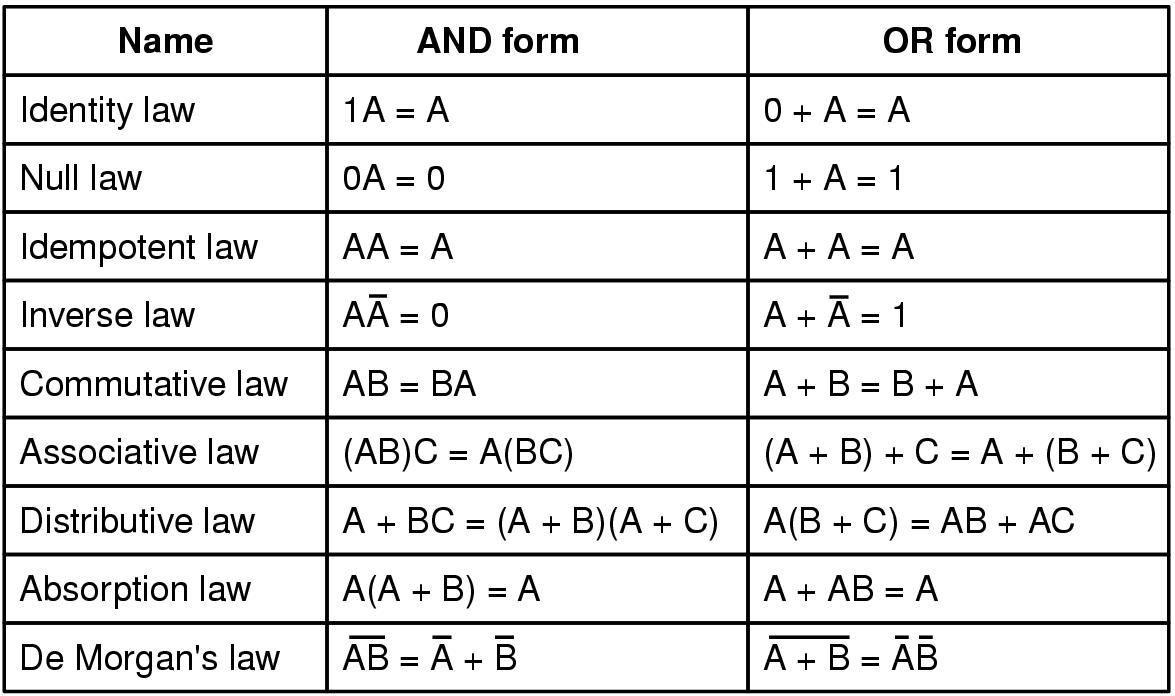
\includegraphics[width=8cm,height=5cm]{figures/logica.png}

    \item* $1$
    \item $A + C$
    \item $B + C$
    \item $\overline{A} + \overline{B}$
\end{multi}

\begin{multi}[points=1,shuffle=true]{Semplificazione di espressioni logiche}
    Semplificare la seguente espressione logica: $(CD + \overline{A}D)C$

    Come riferimento, le seguenti equivalenze logiche sono valide:

    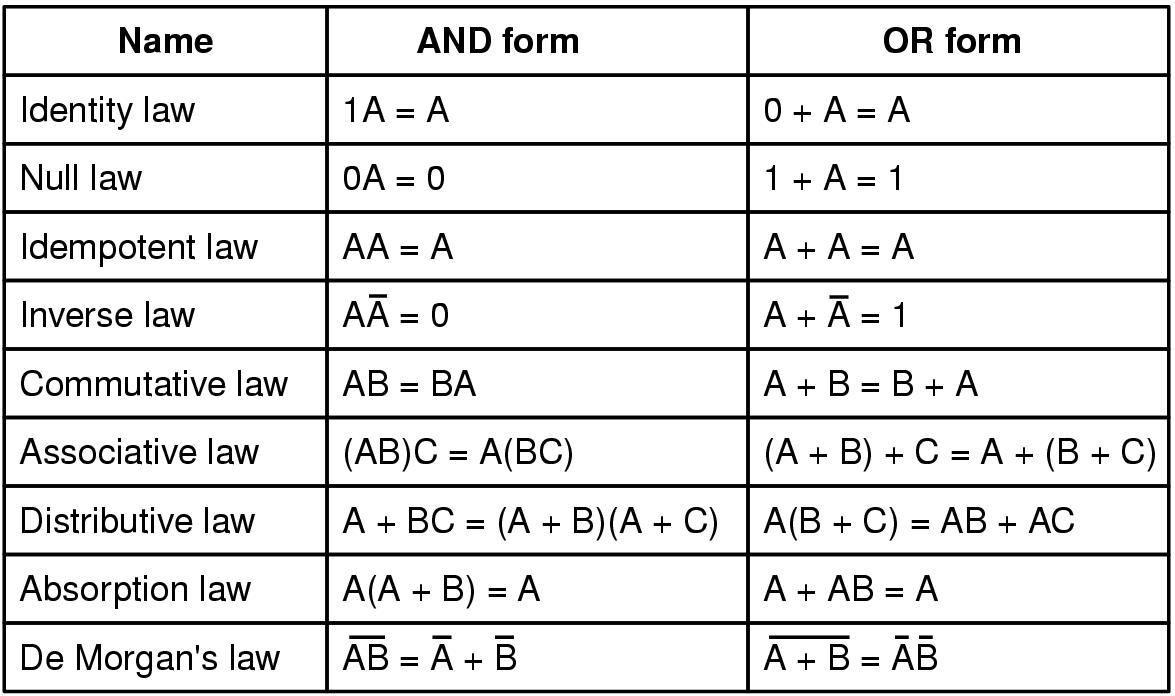
\includegraphics[width=9cm,height=6cm]{figures/logica.png}

    \item* $CD$
    \item $AC$
    \item $B + C$
    \item $\overline{D}B$
\end{multi}

\begin{multi}[points=1,shuffle=true]{Semplificazione di espressioni logiche}
    Semplificare la seguente espressione logica: $ \overline{AB} +  \overline{A}BD$

    Come riferimento, le seguenti equivalenze logiche sono valide:

    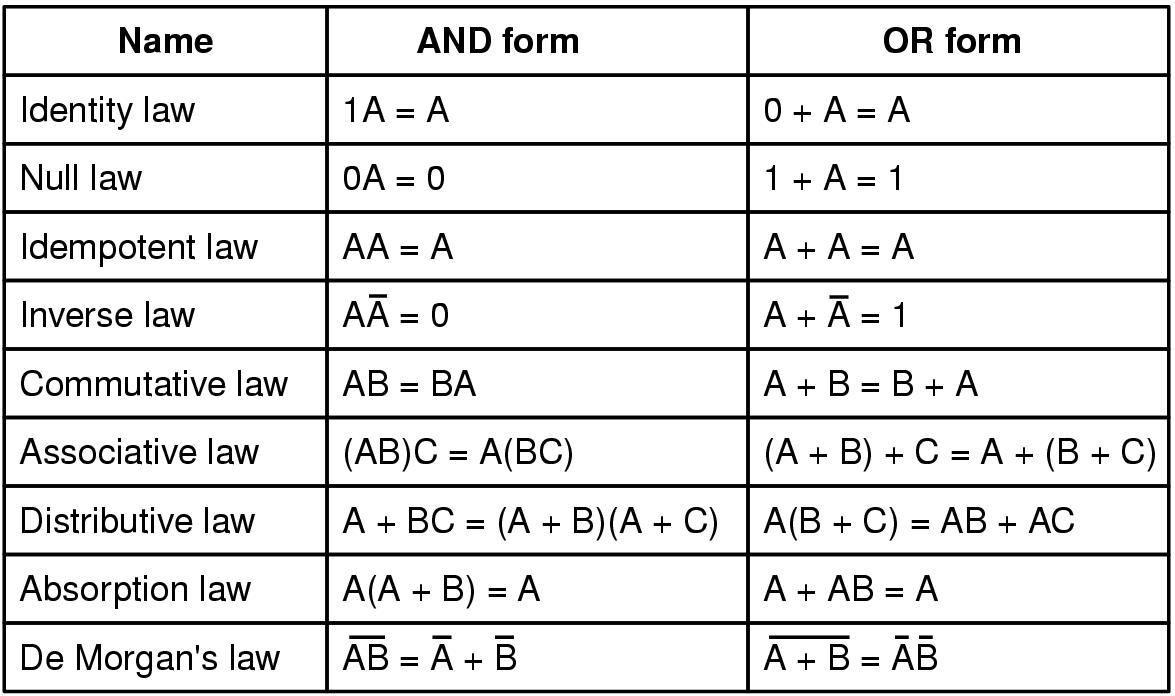
\includegraphics[width=9cm,height=6cm]{figures/logica.png}

    \item* $\overline{A}+\overline{B}$
    \item $AD$
    \item $B + D$
    \item $\overline{A}B$
\end{multi}


\begin{multi}[points=1,shuffle=true]{Semplificazione di espressioni logiche}
    Semplificare la seguente espressione logica: \\
    $C \cdot D + (A + \overline{C \cdot B}) \cdot C$\\

    Come riferimento, le seguenti equivalenze logiche sono valide:\\

    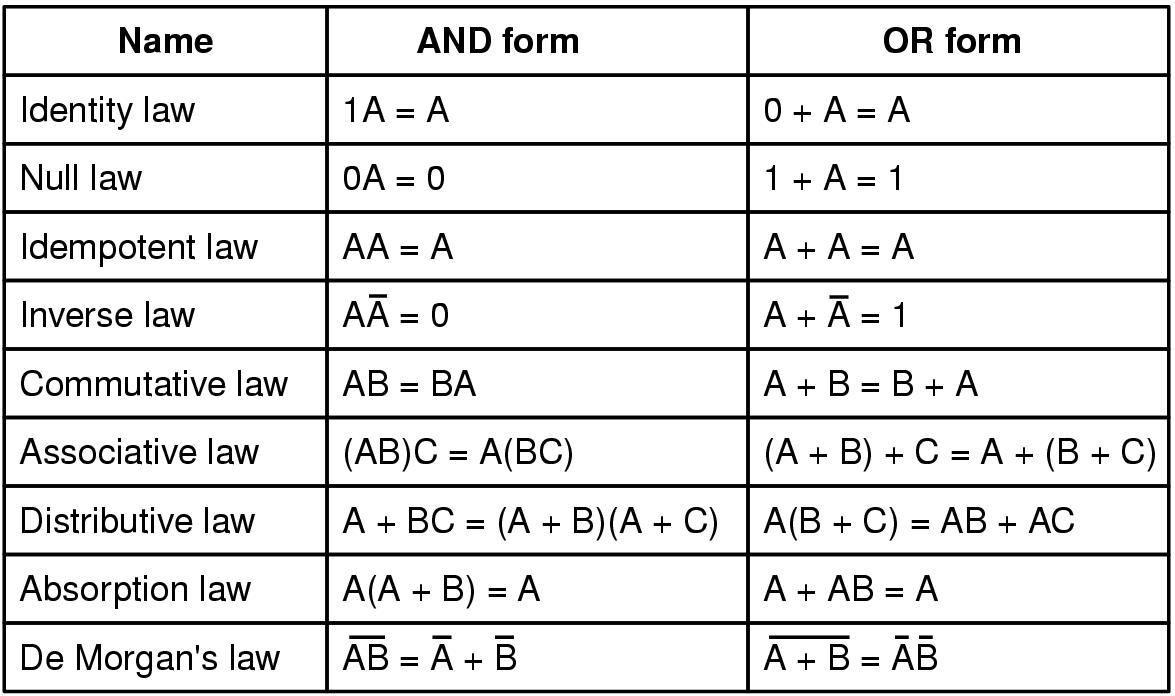
\includegraphics[width=8cm,height=5cm]{figures/logica.png}

    \item* $C \cdot  (A + \overline{B} + D)$
    \item $A \cdot C + \overline{B} +  A \cdot B$
    \item $A \cdot B + \overline{B} + C $
    \item $A + B + D$
\end{multi}

\begin{multi}[points=1,shuffle=true]{Semplificazione di espressioni logiche}
    Semplificare la seguente espressione logica: \\

    $\overline{A} \cdot B + C \cdot (\overline{\overline{B} \cdot C} + D)$\\

    Come riferimento, le seguenti equivalenze logiche sono valide:\\

    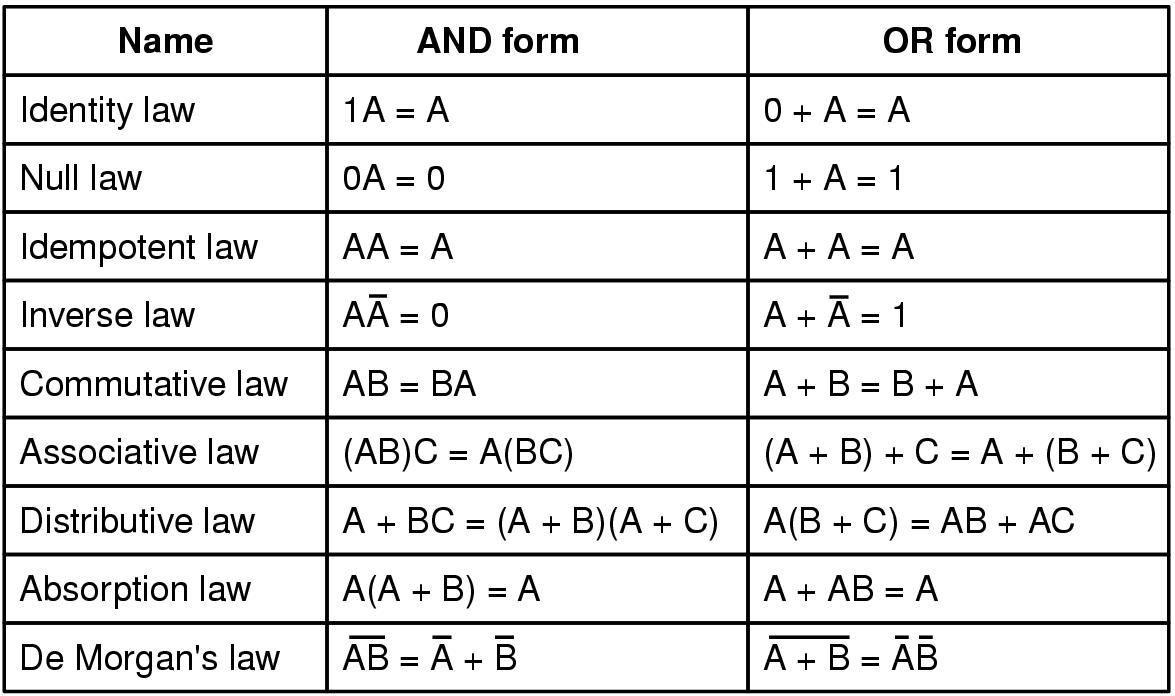
\includegraphics[width=8cm,height=5cm]{figures/logica.png}

    \item* $\overline{A} \cdot B + B \cdot C + C \cdot D$
    \item $\overline{A} \cdot C + B \cdot D + A$
    \item $\overline{B} + C + D$
    \item $\overline{A}  + B \cdot \overline{C} + D$
\end{multi}

\begin{multi}[points=1,shuffle=true]{Da tabella di verita a formula algebrica}
    Determinare la funzione booleana $M$ nella Formula Normale Disgiuntiva (FND) equivalente alla seguente tabella di verit\`{a}.

    $A \qquad  B \qquad  C \quad M$ \\
    $0 \qquad 0 \qquad 0 \qquad 0$ \\
    $0 \qquad 0 \qquad 1 \qquad 0$ \\
    $0 \qquad 1 \qquad 0 \qquad 0$ \\
    $0 \qquad 1 \qquad 1 \qquad 0$ \\
    $1 \qquad 0 \qquad 0 \qquad 1$ \\
    $1 \qquad 0 \qquad 1 \qquad 1$ \\
    $1 \qquad 1 \qquad 0 \qquad 0$ \\
    $1 \qquad 1 \qquad 1 \qquad 1$ \\
    
    \item* $ABC\ +\ A\bar{B}$
    \item $ABC\ +\ A\bar{C}$
    \item $ABC\ +\ \bar{A}B$
    \item $ABC\ +\ \bar{A}\bar{B}$
\end{multi}

\begin{multi}[points=1,shuffle=true]{Da tabella di verita a formula algebrica}
    Determinare la funzione booleana $M$ nella Formula Normale Disgiuntiva (FND) equivalente alla seguente tabella di verit\`{a}.

    $A \qquad  B \qquad  C \quad M$ \\
    $0 \qquad 0 \qquad 0 \qquad 0$ \\
    $0 \qquad 0 \qquad 1 \qquad 0$ \\
    $0 \qquad 1 \qquad 0 \qquad 0$ \\
    $0 \qquad 1 \qquad 1 \qquad 0$ \\
    $1 \qquad 0 \qquad 0 \qquad 1$ \\
    $1 \qquad 0 \qquad 1 \qquad 0$ \\
    $1 \qquad 1 \qquad 0 \qquad 1$ \\
    $1 \qquad 1 \qquad 1 \qquad 1$ \\
    
    \item* $ABC\ +\ A\bar{C}$
    \item $ABC\ +\ \bar{A}B$
    \item $ABC\ +\ \bar{A}\bar{B}$
    \item $ABC\ +\ \bar{A}BC$
\end{multi}

\begin{multi}[points=1,shuffle=true]{Da tabella di verita a formula algebrica}
    Determinare la funzione booleana $M$ nella Formula Normale Disgiuntiva (FND) equivalente alla seguente tabella di verit\`{a}.

    $A \qquad  B \qquad  C \quad M$ \\
    $0 \qquad 0 \qquad 0 \qquad 0$ \\
    $0 \qquad 0 \qquad 1 \qquad 0$ \\
    $0 \qquad 1 \qquad 0 \qquad 1$ \\
    $0 \qquad 1 \qquad 1 \qquad 1$ \\
    $1 \qquad 0 \qquad 0 \qquad 0$ \\
    $1 \qquad 0 \qquad 1 \qquad 0$ \\
    $1 \qquad 1 \qquad 0 \qquad 0$ \\
    $1 \qquad 1 \qquad 1 \qquad 1$ \\
    
    \item* $ABC\ +\ \bar{A}B$
    \item $ABC\ +\ \bar{A}\bar{B}$
    \item $ABC\ +\ \bar{A}BC$
    \item $\bar{A}\bar{B}C\ +\ \bar{A}C$
\end{multi}

\begin{multi}[points=1,shuffle=true]{Da tabella di verita a formula algebrica}
    Determinare la funzione booleana $M$ nella Formula Normale Disgiuntiva (FND) equivalente alla seguente tabella di verit\`{a}.

    $A \qquad  B \qquad  C \quad M$ \\
    $0 \qquad 0 \qquad 0 \qquad 1$ \\
    $0 \qquad 0 \qquad 1 \qquad 1$ \\
    $0 \qquad 1 \qquad 0 \qquad 0$ \\
    $0 \qquad 1 \qquad 1 \qquad 0$ \\
    $1 \qquad 0 \qquad 0 \qquad 0$ \\
    $1 \qquad 0 \qquad 1 \qquad 0$ \\
    $1 \qquad 1 \qquad 0 \qquad 0$ \\
    $1 \qquad 1 \qquad 1 \qquad 1$ \\
    
    \item* $ABC\ +\ \bar{A}\bar{B}$
    \item $ABC\ +\ \bar{A}BC$
    \item $\bar{A}\bar{B}C\ +\ \bar{A}C$
    \item $\bar{A}BC\ +\ A\bar{B}$
\end{multi}

\begin{multi}[points=1,shuffle=true]{Da tabella di verità a formula algebrica}
    Determinare la funzione booleana $M$ nella Formula Normale Congiuntiva (FNC) equivalente alla seguente tabella di verit\`{a}.

    $A \qquad  B \qquad  C \quad M$ \\
    $0 \qquad 0 \qquad 0 \qquad 0$ \\
    $0 \qquad 0 \qquad 1 \qquad 0$ \\
    $0 \qquad 1 \qquad 0 \qquad 1$ \\
    $0 \qquad 1 \qquad 1 \qquad 1$ \\
    $1 \qquad 0 \qquad 0 \qquad 1$ \\
    $1 \qquad 0 \qquad 1 \qquad 1$ \\
    $1 \qquad 1 \qquad 0 \qquad 1$ \\
    $1 \qquad 1 \qquad 1 \qquad 1$ \\
    
    \item* $(A\ +\ B\ +\ C)(A\ +\ B\ +\ \bar{C})$
    \item $(A\ +\ B\ +\ C)(A\ +\ \bar{B}\ +\ C)$
    \item $(A\ +\ B\ +\ C)(\bar{A}\ +\ B\ +\ C)$
    \item $(\bar{A}\ +\ B\ +\ C)(A\ +\ B\ +\ \bar{C})$
\end{multi}

\begin{multi}[points=1,shuffle=true]{Da tabella di verità a formula algebrica}
    Determinare la funzione booleana $M$ nella Formula Normale Congiuntiva (FNC) equivalente alla seguente tabella di verit\`{a}.

    $A \qquad  B \qquad  C \quad M$ \\
    $0 \qquad 0 \qquad 0 \qquad 0$ \\
    $0 \qquad 0 \qquad 1 \qquad 1$ \\
    $0 \qquad 1 \qquad 0 \qquad 0$ \\
    $0 \qquad 1 \qquad 1 \qquad 1$ \\
    $1 \qquad 0 \qquad 0 \qquad 1$ \\
    $1 \qquad 0 \qquad 1 \qquad 1$ \\
    $1 \qquad 1 \qquad 0 \qquad 1$ \\
    $1 \qquad 1 \qquad 1 \qquad 1$ \\
    
    \item* $(A\ +\ B\ +\ C)(A\ +\ \bar{B}\ +\ C)$
    \item $(A\ +\ B\ +\ C)(\bar{A}\ +\ B\ +\ C)$
    \item $(\bar{A}\ +\ B\ +\ C)(A\ +\ B\ +\ \bar{C})$
    \item $(\bar{A}\ +\ B\ +\ C)(A\ +\ \bar{B}\ +\ C)$
\end{multi}

\begin{multi}[points=1,shuffle=true]{Da tabella di verità a formula algebrica}
    Determinare la funzione booleana $M$ nella Formula Normale Congiuntiva (FNC) equivalente alla seguente tabella di verit\`{a}.

    $A \qquad  B \qquad  C \quad M$ \\
    $0 \qquad 0 \qquad 0 \qquad 0$ \\
    $0 \qquad 0 \qquad 1 \qquad 1$ \\
    $0 \qquad 1 \qquad 0 \qquad 1$ \\
    $0 \qquad 1 \qquad 1 \qquad 1$ \\
    $1 \qquad 0 \qquad 0 \qquad 0$ \\
    $1 \qquad 0 \qquad 1 \qquad 1$ \\
    $1 \qquad 1 \qquad 0 \qquad 1$ \\
    $1 \qquad 1 \qquad 1 \qquad 1$ \\
    
    \item* $(A\ +\ B\ +\ C)(\bar{A}\ +\ B\ +\ C)$
    \item $(\bar{A}\ +\ B\ +\ C)(A\ +\ B\ +\ \bar{C})$
    \item $(\bar{A}\ +\ B\ +\ C)(A\ +\ \bar{B}\ +\ C)$
    \item $(\bar{A}\ +\ \bar{B}\ +\ C)(A\ +\ B\ +\ \bar{C})$
\end{multi}

\begin{multi}[points=1,shuffle=true]{Da tabella di verità a formula algebrica}
    Determinare la funzione booleana $M$ nella Formula Normale Congiuntiva (FNC) equivalente alla seguente tabella di verit\`{a}.

    $A \qquad  B \qquad  C \quad M$ \\
    $0 \qquad 0 \qquad 0 \qquad 1$ \\
    $0 \qquad 0 \qquad 1 \qquad 0$ \\
    $0 \qquad 1 \qquad 0 \qquad 1$ \\
    $0 \qquad 1 \qquad 1 \qquad 1$ \\
    $1 \qquad 0 \qquad 0 \qquad 0$ \\
    $1 \qquad 0 \qquad 1 \qquad 1$ \\
    $1 \qquad 1 \qquad 0 \qquad 1$ \\
    $1 \qquad 1 \qquad 1 \qquad 1$ \\
    
    \item* $(\bar{A}\ +\ B\ +\ C)(A\ +\ B\ +\ \bar{C})$
    \item $(\bar{A}\ +\ B\ +\ C)(A\ +\ \bar{B}\ +\ C)$
    \item $(\bar{A}\ +\ \bar{B}\ +\ C)(A\ +\ B\ +\ \bar{C})$
    \item $(\bar{A}\ +\ \bar{B}\ +\ C)(\bar{A}\ +\ B\ +\ \bar{C})$
\end{multi}

\begin{multi}[points=1,shuffle=true]{Reti combinatorie}
    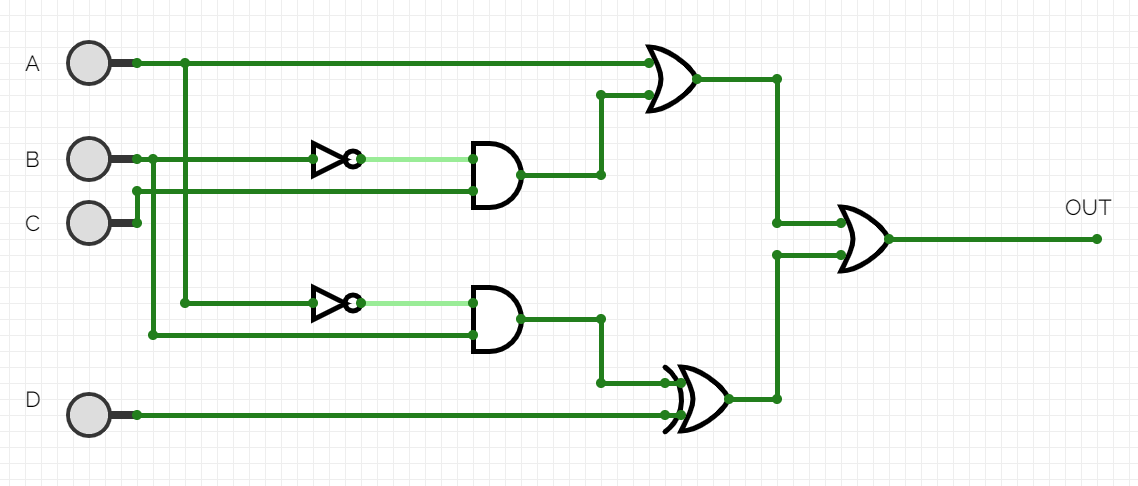
\includegraphics[height=6cm]{figures/comb1.png}

    Data la rete combinatoria mostrata in figura, determinare l'espressione logica relativa all'uscita OUT (NOTA: $\oplus$ rappresenta l'operatore $XOR$):

    \item $(A+ \overline{C}A)+((AB) \oplus C)$
    \item* $(A+ \overline{B}C)+((\overline{A}B) \oplus D)$
    \item $(\overline{C}\oplus A)+((\overline{A}B) + C)$
    \item $ABC+ \overline{B \oplus D}$
\end{multi}

\begin{multi}[points=1,shuffle=true]{Reti combinatorie}
    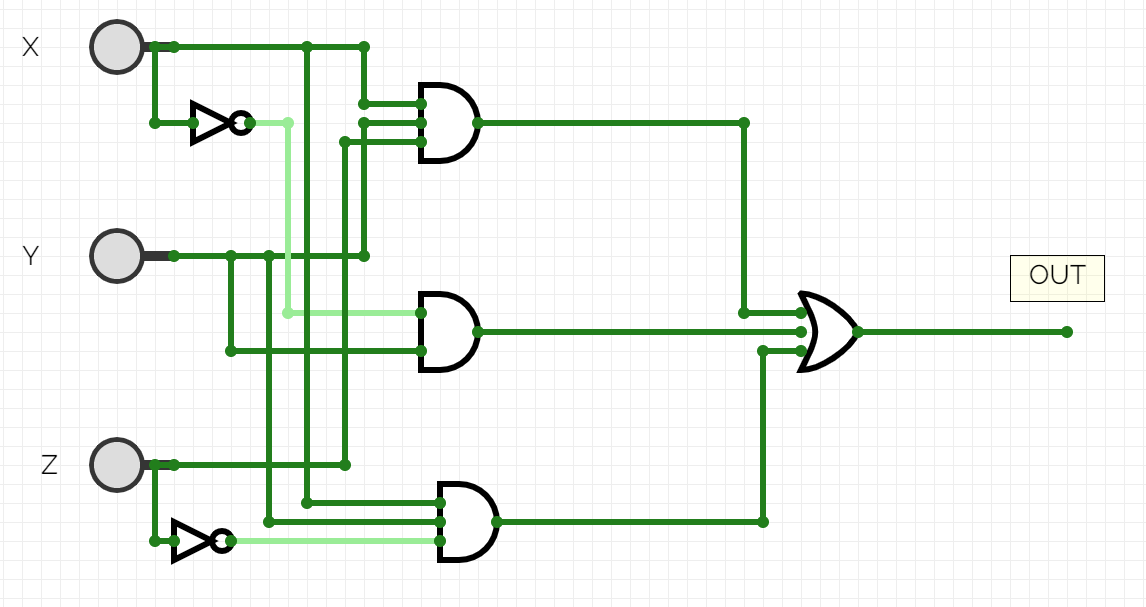
\includegraphics[height=6.5cm]{figures/comb2.png}

    Data la rete combinatoria mostrata in figura, determinare l'espressione logica relativa all'uscita OUT:

    \item* $Y(XZ+ \overline{X}+X \overline{Z})$
    \item $YZ + X\overline{Y} +\overline{X}YZ$
    \item $\overline{XZ} + \overline{Y}XZ + Y\overline{Z}$
    \item $Z(YX+ \overline{XY}+ \overline{Y})$
\end{multi}

\begin{multi}[points=1,shuffle=true]{Reti combinatorie}
    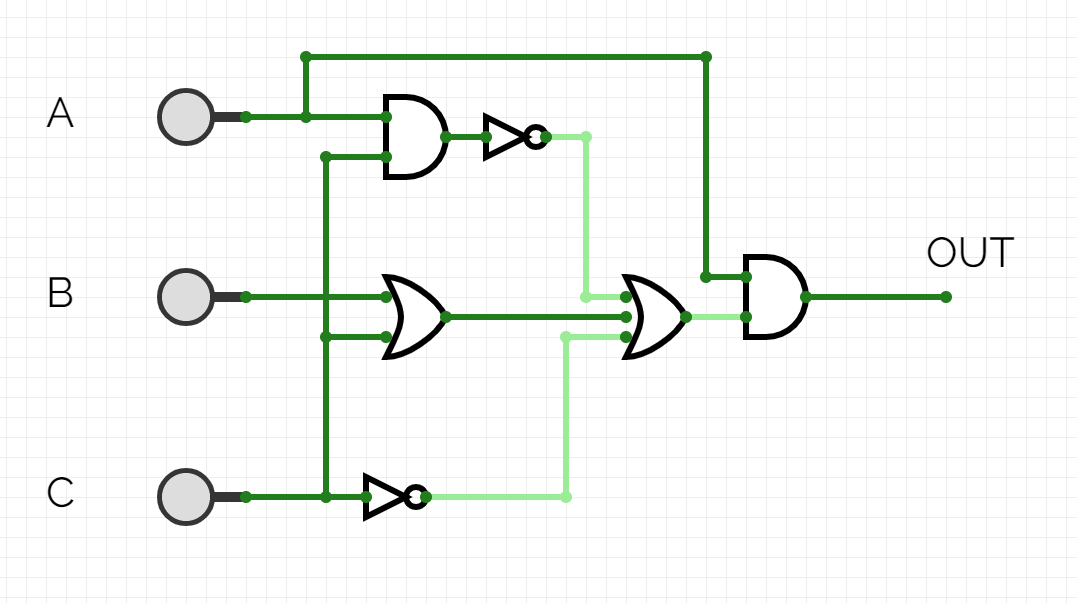
\includegraphics[height=6cm]{figures/comb3.png}

    Data la rete combinatoria mostrata in figura, determinare l'espressione logica relativa all'uscita OUT:

    \item* $A$
    \item $(\overline{BC}+A)B$
    \item $(\overline{AB}+C)A$
    \item $(\overline{C}+AB)C$
\end{multi}

\end{quiz}
\end{document}